\newcommand{\touche}[1]{{
\begin{picture}(12,12)(0, 2)
\put(0,0){\framebox(12,12)[lb]{}}
\put(1.5,2){\makebox(0,0)[lb]{\tiny #1}}
\end{picture}\hspace{0.3ex}}}


\section{The robot}
%\label{sec:2:le-robot}

To make our geometric drawings on the computer we are going to drive
a little robot. Its name is \robot\@\footnote{\ The way its name is written
leaves no doubt about its humanoid and friendly nature.
}. To draw with the \robot, double-click on its icon
\begin{center}
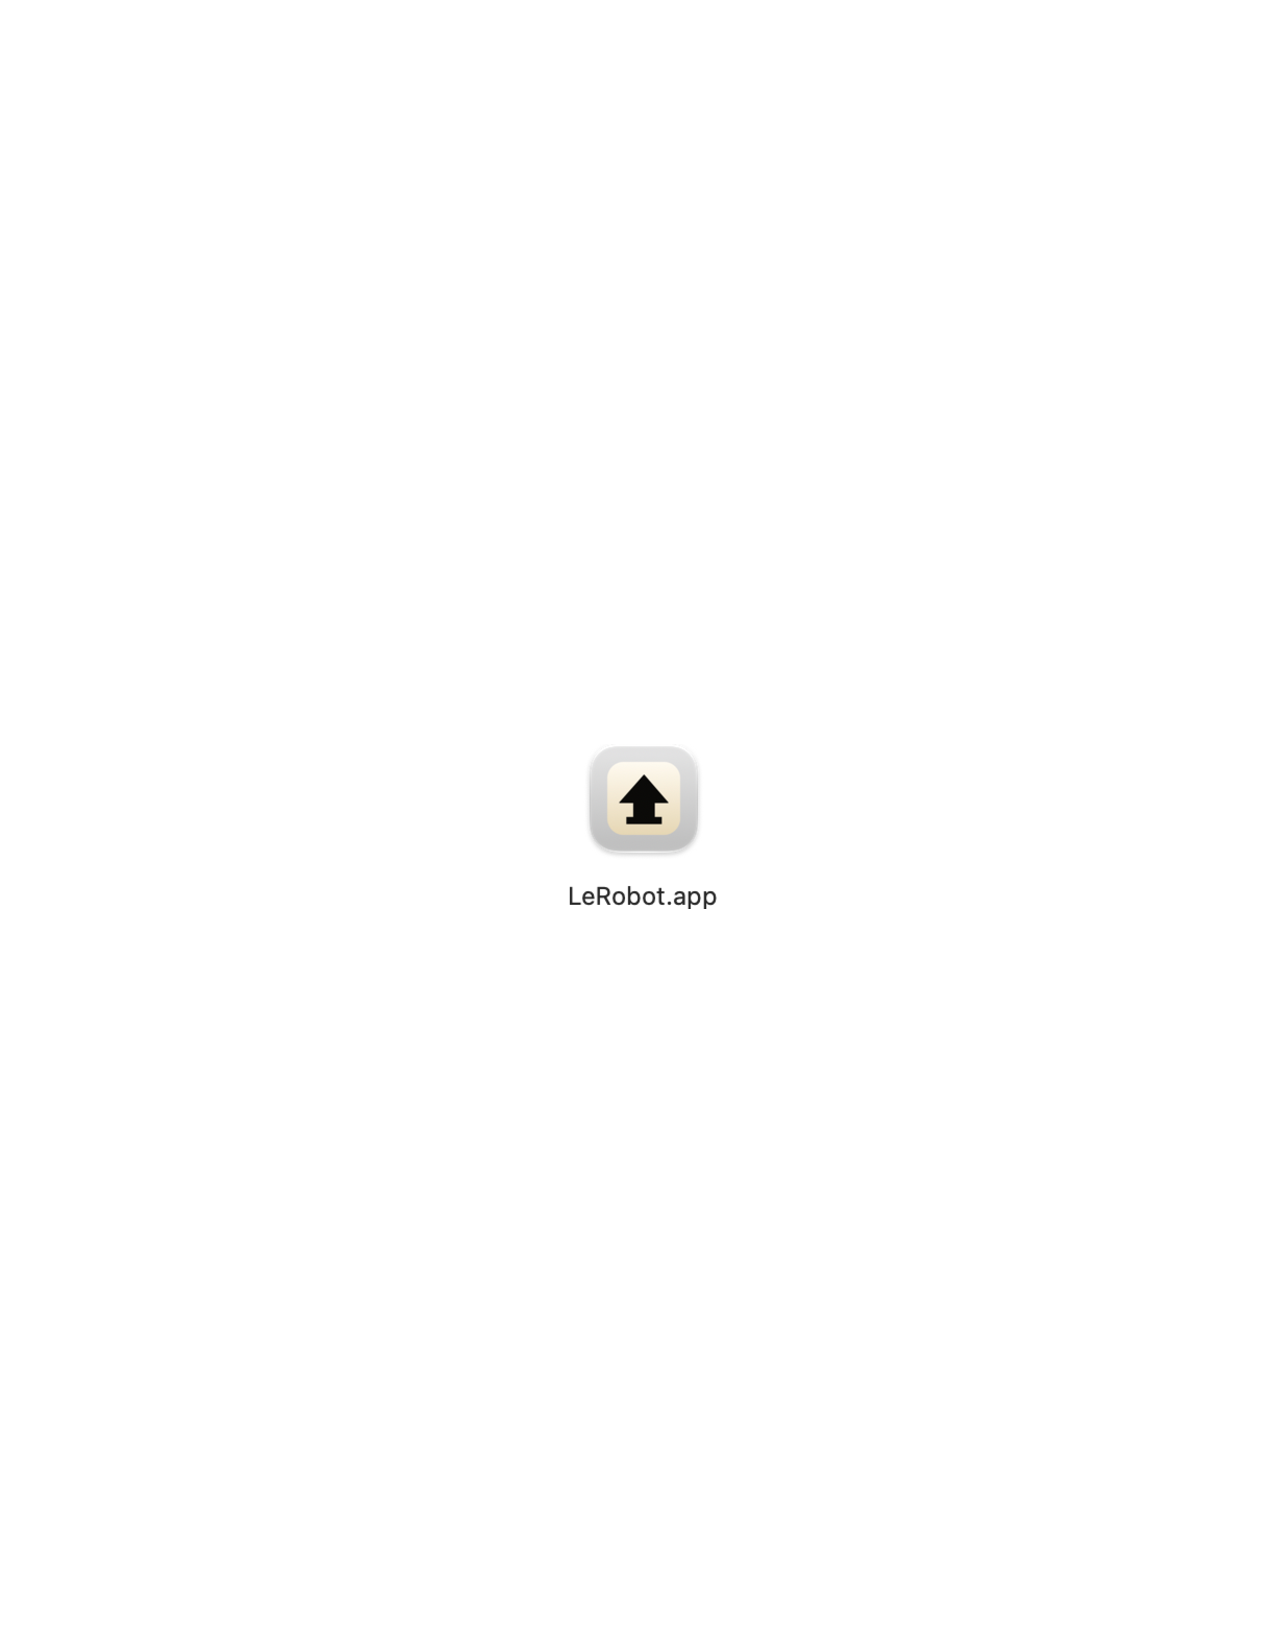
\includegraphics[scale=0.6]{ps-files/LeRobotAppIcone}
\end{center}
Our \robot\ carries a pen which it can raise or
lower while it moves about on the computer screen.
When the \robot\
moves with its pen down, it leaves a trail on the screen,
just as a snail would on a sheet of paper. When it moves with its
pen up, it leaves no trace of where it has been.  To draw,
the \robot\ must follow the lines of the drawing exactly with its pen
down.
It can also go from one point of the drawing to another point which is not
joined to it by a line by raising its pen. To guide the
\robot\ we use the computer keyboard, which serves as a remote control.
So we can drive the \robot\ as if it were a little
radio-controlled car.

\smallskip

On the computer screen our \robot\ is represented by a
small arrow \robotCbN\ which shows in which direction of the
compass rose it is facing (see figure
\ref{fig:rose-des-vents-8d}, page \pageref{fig:rose-des-vents-8d}). It can face
north \robotCbN\/, north-east \robotCbNE, east \robotCbE\/,
south-east \robotCbSE\/, south \robotCbS\/, south-west \robotCbSW\/,
west \robotCbW\ or north-west \robotCbNW\/.
The arrow is solid when the \robot\ has lowered its pen and
hollow
(\robotClN\/, \robotClNE\/, \robotClE\/, \robotClSE\/, \robotClS\/,
\robotClSW\/,  \robotClW\ or \robotClNW\/) when the pen is up.
\begin{figure}[htbp]
 \includehvspacePostScript[6cm,5.6cm]{rose-des-vents-8d}{0.95}{0.95}
 \caption{Eight-point compass rose}\label{fig:rose-des-vents-8d}
\end{figure}

\smallskip

Like trains on their rails, our \robot\ cannot go
just anywhere on the screen. It must always move along
the lines or arcs joining two successive points of a grid whose size is
fixed by the size of the computer screen. A small part of this grid
is shown \hbox{below} in figure \ref{fig:grille}.
\index{Grid of the robot@Grid of the \protect\smash{\protect\robot}}%
\begin{figure}[htbp]
 \includehvspacePostScript[\textwidth,4.0cm]{grille}{0.95}{0.95}
 \caption{Grid and stopping points of the \protect\robot}
 \label{fig:grille}
\end{figure}

\noindent This imaginary grid corresponds to the squared paper we used to
make our drawings by hand, except that the squares are not visible on
the computer screen.
After a move, the \robot\ always stops at the intersection
of a horizontal line and a vertical line of the imaginary grid. Figure
 \ref{fig:traject} (page \pageref{fig:traject}) shows all the possible paths
of the \robot\ between any two stopping points on the grid.
\begin{figure}[htbp]
 \includevspacePostScript[5.4cm]{dessincomplexe}{0.95}{0.95}
 \caption{Paths of the \protect\robot\ (magnification $\times$\ $4.5$)}
 \label{fig:traject}
\end{figure}
\begin{figure}[htbp]
 \includehvspacePostScript[42mm,2.1cm]{robot-arrete}{0.95}{0.95}
 \caption{The \protect\robot\ at rest (magnification $\times$\ $2.5$)}
 \label{fig:robot-arrete}
\end{figure}
Figure \ref{fig:robot-arrete} \hbox{(page \pageref{fig:robot-arrete})}
shows the exact
position of the \robot\ when it stops on the grid. It places the tip of
its pen, located in the middle at the back of the arrow, exactly on
a stopping point of the grid.


\section{Driving the robot}

To drive the \robot\ on the computer, you must ``{\em run the program}
{\idt Draw}'', which is part of the {\idt LeRobot\_Python\_EN} library
that comes with this book%
\footnote{\ Just double-click on the icon of the \robot\ {\tt LeRobotPythonEN.app}.
You can also, in a terminal window opened in the folder
{\tt LeRobot\_Python\_EN}, type
{\tt python3 Draw.py}. On the Macintosh, the window of the \robot\ is an
ordinary window, which comes to the front; if the keys have no effect, click
in this window.}.

\subsection{Initial position of the robot}

When the program {\idt Draw}
starts running, the computer
screen looks as shown, reduced, in figure
\ref{fig:ecran-initial-1}  (page \pageref{fig:ecran-initial-1}).
\begin{figure}[htbp]
 \includevspacePostScript[7.6cm]{ecran-initial-1}{0.95}{0.95}
 \caption{The computer screen at the start}
 \centering{of the execution of the program {\idt Draw}}
 \label{fig:ecran-initial-1}
\end{figure}
So at the start the \robot\ is at rest in the middle of the imaginary
grid, with its pen down, facing north \robotCbN\/.
To drive the \robot, we use the keys of the computer keyboard,
which serves as a remote control. We shall now
see which keys to press to raise or lower the pen,
move forward, turn on the spot, make a turn, etc.

\subsection{Handling the robot's pen}

 By pressing the key marked \touche{U} on the
keyboard, the \robot\ raises its pen \robotClN\/. By pressing the key
\touche{D}, it lowers it \robotCbN\/. As there is not much room on the computer
screen to
recall the instructions for the \robot\ in detail, we use
mnemonic abbreviations%
%
\footnote{\ Mnemonic abbreviations help the memory by association of ideas.}
placed at the bottom of the screen, as can be
seen in figure
\ref{fig:ecran-initial-1} above.
These abbreviations are made of the first letters of English words.
For \hbox{example:}
\begin{list}{$\scriptscriptstyle\bullet$}{
}
\item {\idt u}\,$:${\idt pu} means ``the key \touche{U} raises the pen'':
\hbox{\underline{p}en \underline{u}p;}
\item {\idt d}\,$:${\idt pd} means ``the key \touche{D} lowers the pen'':
\hbox{\underline{p}en \underline{d}own.}
\end{list}
Letters are typed in lower case, without pressing the shift key
(a capital letter is not a command of the \robot).

The effect of the keys \touche{U} and \touche{D} that handle the pen of the
\robot\ is summarised in table \ref{tab:crayon} (page \pageref{tab:crayon}).

\begin{table}[htbp]
\begin{center}
\begin{tabular}{@{}|c|c|c|c|c|c|c|c|c|c|@{}} \hline
\touche{U} ({\idt pu}) & Before   & \robotCbN  & \robotCbNE & \robotCbE & \robotCbSE & \robotCbS  & \robotCbSW
& \robotCbW & \robotCbNW \\ \cline{2-10}
                     & After & \robotClN  & \robotClNE & \robotClE & \robotClSE  & \robotClS
& \robotClSW & \robotClW  & \robotClNW  \\ \hline\hline
\touche{D} ({\idt pd}) & Before  & \robotClN  & \robotClNE & \robotClE & \robotClSE & \robotClS  & \robotClSW
& \robotClW  & \robotClNW  \\ \cline{2-10}
                         & After & \robotCbN & \robotCbNE & \robotCbE  & \robotCbSE   & \robotCbS
& \robotCbSW & \robotCbW  & \robotCbNW \\ \hline
\end{tabular}
\end{center}
\caption{Handling the pen of the \protect\robot}
\label{tab:crayon}
\end{table}



\subsection{Turning the robot a quarter turn on the spot}


The key \touche{$-$} turns the \robot\ on the spot a quarter turn to the left
({\idt qtl} for short, from
\underline{q}uarter \underline{t}urn \underline{l}eft).
For example, if the \robot\ is facing north \robotCbN\/, the key \touche{$-$}
turns it on the spot to face west \robotCbW\/. If it is facing east \robotCbE\/,
it turns to face north \robotCbN\/.
The key \touche{$+$} turns the \robot\ on the spot a quarter turn to the right
({\idt qtr} for short, from
\underline{q}uarter \underline{t}urn \underline{r}ight).

When we speak of the left side of the \robot, you must imagine yourself in
the place of the \robot, looking in the direction of
the arrow. For example, the left of \robotCbE\ is the top of this page, whereas
the left of \robotCbS\ is on the right of this \hbox{sheet!}

The effect of the commands \touche{$-$} ({\idt qtl})  and \touche{$+$} ({\idt qtr})
is summarised in the table below for the case where the pen is down. The effect is
the same when the pen is up.
\begin{table}[htbp]
\begin{center}
\begin{tabular}{@{}|c|c|c|c|c|c|c|c|c|c|@{}} \hline
\touche{$-$} ({\idt qtl}) & Before   & \robotCbN & \robotCbNE & \robotCbE & \robotCbSE & \robotCbS & \robotCbSW & \robotCbW & \robotCbNW \\ \cline{2-10}
                         & After & \robotCbW & \robotCbNW & \robotCbN & \robotCbNE & \robotCbE & \robotCbSE & \robotCbS & \robotCbSW \\ \hline \hline
\touche{$+$} ({\idt qtr}) & Before   & \robotCbN & \robotCbNE & \robotCbE & \robotCbSE & \robotCbS & \robotCbSW & \robotCbW & \robotCbNW \\ \cline{2-10}
                         & After & \robotCbE & \robotCbSE & \robotCbS & \robotCbSW & \robotCbW & \robotCbNW & \robotCbN & \robotCbNE \\ \hline
\end{tabular}
\end{center}
\caption{Quarter turns of the \protect\robot\ on the spot}
%\label{tab:pqtdg}
\end{table}

\subsection{Turning the robot an eighth turn on the spot}

The key \touche{L} turns the \robot\ on the spot an eighth turn to the left
({\idt etl} for short, from
\underline{e}ighth \underline{t}urn \underline{l}eft; the key {\tt L} stands for ``left'').
For example, if it is facing north \robotCbN\/, the \robot\ turns to face
north-west \robotCbNW\/. If you keep pressing the key \touche{L}, the \robot\
turns an eighth turn each time, going through the successive positions
\robotCbW\ then \robotCbSW\/, \robotCbS\/, \robotCbSE\/, \robotCbE\/, \robotCbNE\/, \ldots
The key \touche{R} turns the \robot\ on the spot an eighth turn to the right
({\idt etr} for short, from
\underline{e}ighth \underline{t}urn \underline{r}ight; {\tt R} stands for ``right'').
The effect of the keys  \touche{L} ({\idt etl})  and \touche{R} ({\idt etr}) is summarised
\hbox{below:}
\begin{table}[htbp]
\begin{center}
\begin{tabular}{@{}|c|c|c|c|c|c|c|c|c|c|@{}} \hline
\touche{L} ({\idt etl}) & Before    & \robotCbN  & \robotCbNW & \robotCbW  & \robotCbSW & \robotCbS  & \robotCbSE & \robotCbE  & \robotCbNE \\ \cline{2-10}
                       & After  & \robotCbNW & \robotCbW  & \robotCbSW & \robotCbS  & \robotCbSE &\robotCbE   & \robotCbNE & \robotCbN  \\ \hline \hline
\touche{R} ({\idt etr}) & Before    & \robotCbN  & \robotCbNE & \robotCbE  & \robotCbSE & \robotCbS  & \robotCbSW & \robotCbW  & \robotCbNW \\ \cline{2-10}
                       & After & \robotCbNE & \robotCbE  & \robotCbSE & \robotCbS  & \robotCbSW & \robotCbW  & \robotCbNW & \robotCbN  \\ \hline
\end{tabular}
\end{center}
\caption{Eighth turns of the \protect\robot\ on the spot}
%\label{tab:phtgd}
\end{table}

\subsection{Moving the robot forward}

The key \touche{F} makes the \robot\ move straight forward by the length of one
side of a square of the grid.
The mnemonic abbreviation of this command of the \robot\ is {\idt fd}, from
\underline{f}orwar\underline{d} (and {\tt F} is the first letter of ``forward'').
If the pen is down, this move draws a short line. If the pen
is up, this move leaves no trace on the drawing. In both cases the
\robot\ moves straight ahead in the direction it is facing without
changing \hbox{direction:}
\begin{table}[htbp]
\begin{center}
\input ROBOT-AVPICT2.46x2.46.tex
\input ROBOT+AVPICT2.46x2.46.tex
\input ROBOT-VGPICT2.46x2.46.tex
\input ROBOT+VGPICT2.46x2.46.tex
\input ROBOT-VDPICT2.46x2.46.tex
\input ROBOT+VDPICT2.46x2.46.tex
\begin{tabular}{@{}|c|c|c|c|c|c|c|c|c|c|@{}} \hline
\touche{F} ({\idt fd}) & Before   & \robotCbNmav & \robotCbNEmav & \robotCbEmav & \robotCbSEmav & \robotCbSmav & \robotCbSWmav & \robotCbWmav & \robotCbNWmav \\ \cline{2-10}
                     & After & \robotCbNpav & \robotCbNEpav & \robotCbEpav & \robotCbSEpav & \robotCbSpav & \robotCbSWpav & \robotCbWpav & \robotCbNWpav \\ \hline
\end{tabular}
\end{center}
\caption{Forward moves of the \protect\robot\ in the eight directions}
%\label{tab:av-8d}
\end{table}

\begin{exemple}[Notched frieze]{\rm
 By pressing the keys \touche{F} ({\idt fd}), \touche{$+$} ({\idt qtr}),  \touche{F} ({\idt fd}),
\touche{$+$} ({\idt qtr}), \touche{F} ({\idt fd}), \touche{$-$} ({\idt qtl}), \touche{F} ({\idt fd}),
\touche{$-$} ({\idt qtl}), \touche{F} ({\idt fd}), \touche{$+$} ({\idt qtr}),  \touche{F} ({\idt fd}),
\touche{$+$} ({\idt qtr}), \touche{F} ({\idt fd}), \touche{$-$} ({\idt qtl}), \touche{F} ({\idt fd}),
\touche{$-$} ({\idt qtl}), \ldots\ one after the other, we get the \hbox{following frieze:}

\includevspacePostScript[0.7cm]{frise-crantee}{0.95}{0.95}
\noindent $\Box$ }\end{exemple}

\begin{exemple}[Battlement frieze]{\rm
 By pressing the keys
\touche{R} ({\idt etr}), \touche{R} ({\idt etr}), \touche{F} ({\idt fd}), \touche{R} ({\idt etr}),
\touche{F} ({\idt fd}), \touche{L} ({\idt etl}), \touche{F} ({\idt fd}), \touche{L} ({\idt etl}),
\touche{F} ({\idt fd}), \touche{R} ({\idt etr}), \touche{F} ({\idt fd}), \touche{R} ({\idt etr}),
\touche{F} ({\idt fd}), \ldots\ one after the other, we get the \hbox{following frieze:}

\includevspacePostScript[0.7cm]{frise-crenelee}{0.95}{0.95}
\noindent $\Box$ }\end{exemple}

\subsection{Making the robot turn along an arc}

The key \touche{(} \vspace{-1.0mm} makes the \robot\ turn to the left along an arc
({\idt cl} for short, from \underline{c}urve \underline{l}eft) whereas the
key \touche{)} makes it turn to the right along an arc
({\idt cr}, \underline{c}urve \underline{r}ight).
These keys were
chosen because parentheses suggest the idea of a bend and
the left parenthesis \touche{(}, which is on the left of the keyboard,
corresponds to the left turn, whereas the
right parenthesis \touche{)}, which corresponds to the right turn, is on the right of the
keyboard. If the pen is down, this move draws
a small arc of a circle. If the pen is up, this move leaves
no trace on the drawing. In both cases the \robot\ moves on the
grid and changes direction as shown in the table
\hbox{below:}
\begin{table}[htbp]
\begin{center}
\input ROBOT-AVPICT2.46x2.46.tex
\input ROBOT+AVPICT2.46x2.46.tex
\input ROBOT-VGPICT2.46x2.46.tex
\input ROBOT+VGPICT2.46x2.46.tex
\input ROBOT-VDPICT2.46x2.46.tex
\input ROBOT+VDPICT2.46x2.46.tex
\begin{tabular}{@{}|c|c|c|c|c|c|c|c|c|c|@{}} \hline
\touche{(} ({\idt cl}) & Before & \robotCbNmvg & \robotCbNEmvg & \robotCbEmvg & \robotCbSEmvg & \robotCbSmvg & \robotCbSWmvg & \robotCbWmvg & \robotCbNWmvg \\\cline{2-10}
                       & After & \robotCbNpvg & \robotCbNEpvg & \robotCbEpvg & \robotCbSEpvg & \robotCbSpvg & \robotCbSWpvg & \robotCbWpvg & \robotCbNWpvg \\\hline \hline
\touche{)} ({\idt cr}) & Before & \robotCbNmvd & \robotCbNEmvd & \robotCbEmvd & \robotCbSEmvd & \robotCbSmvd & \robotCbSWmvd & \robotCbWmvd & \robotCbNWmvd \\\cline{2-10}
                       & After & \robotCbNpvd & \robotCbNEpvd & \robotCbEpvd & \robotCbSEpvd & \robotCbSpvd & \robotCbSWpvd & \robotCbWpvd & \robotCbNWpvd \\\hline
\end{tabular}
\end{center}
 \caption{Turns of the \protect\robot\ along an arc}
%\label{tab:()-vgd}
\end{table}

\begin{exemple}[Frieze of braces]{\rm
 By pressing the keys
 \touche{)} ({\idt cr}), \touche{(} ({\idt cl}),
 \touche{$+$} ({\idt qtr}), \touche{$+$} ({\idt qtr}),
 \touche{(} ({\idt cl}), \touche{)} ({\idt cr}),
 \touche{$+$} ({\idt qtr}), \touche{$+$} ({\idt qtr}),
 \touche{)} ({\idt cr}), \touche{(} ({\idt cl}),
 \touche{$+$} ({\idt qtr}), \touche{$+$} ({\idt qtr}),
\ldots\ one after the other, we get the \hbox{following frieze:}

\includevspacePostScript[1.0cm]{frise-accolades}{0.95}{0.95}
\noindent $\Box$}\end{exemple}

\subsection{No way out of the frame}

By pressing the key  \touche{F} several times in a row, the \robot\ \robotCbN\ moves straight ahead
drawing a line until it reaches the edge of the frame that bounds its field of action.
If we keep pressing the key
\touche{F} to try to make it leave the frame, this is an {\em error}
in the sense that
the \robotErr\ refuses to do it and gives a
``beep-beep''
of
protest\@\footnote{\ The way its name is written
leaves no doubt about its displeasure.
} (it also writes
``{\tt ** EXIT FORBIDDEN **}''
in the terminal window)!

\subsection{Correcting driving errors}

\index{Error} We often make mistakes when driving the \robotErr. For
example, instead of making it turn to the right with a
right parenthesis \touche{)} ({\idt cr}), we type a left parenthesis
\touche{(} ({\idt cl}) and the \robotErr\ turns
to the left! The {\em delete} key, marked with an arrow
pointing to the left \index{Delete key}
\hspace{0.3ex}\framebox[11.mm][l]{$\leftarrow$~~~}\hspace{0.3ex}
or \hspace{0.3ex}\framebox[11.mm][l]{~~\tiny\texttt{delete}}\hspace{0.3ex},
lets us correct errors by going backwards and erasing
the last lines in the reverse order in which they were
drawn by the \robot.

\subsection{Finishing and reproducing the drawing}

While the program {\idt Draw} is running,
it is possible, at any moment, to
finish the drawing by pressing the return key
\hbox{\framebox[11.mm][l]{$\hookleftarrow$~~~}\hspace{0.3ex}}
or \hspace{0.3ex}\framebox[11.mm][l]{~~\tiny\texttt{return}}\hspace{0.3ex}, also
marked {\small\tt Enter} or {\small\tt Ret} on some computer keyboards ({\small\tt Entrée} on French ones). This is recalled
at the bottom right of the computer screen by a blinking symbol
$\hookleftarrow$.

The drawing that has just been finished is not lost: it is
possible to reproduce it and to print it%
\footnote{\ After the return key, the \robot\ asks in the bottom line
of the screen {\tt Do you want to save in my\_drawing.py? (y/n)}. By pressing
the key \touche{Y}, the drawing is saved as a \python\ program in
the file {\tt my\_drawing.py}, which begins with {\mcl from}\ {\idt LeRobot}\ {\mcl import}\ {\idt *};
it is reproduced by typing {\tt make my\_drawing} (or {\tt python3 my\_drawing.py}) in
the folder {\tt LeRobot\_Python\_EN}. The next drawing saved will replace this file: to keep
the file for good, you must rename it and then run it by dragging it onto the application
\texttt{LeRobotPythonEN.app}.}.


\subsection{Drawing a point, a cross, the grid of the robot's stopping points}

The key \touche{P} ({\idt dp}, \underline{d}raw a \underline{p}oint)
draws a point, without moving the \robot. We use the
key \touche{C} ({\idt dc}, \underline{d}raw a \underline{c}ross)
to draw a small cross {\tt +}. The key \touche{.} ({\idt dg},
\underline{d}raw the \underline{g}rid)
draws the grid of the stopping points
of the \robot\ as can be seen for example in figure
\ref{fig:transports} (page \pageref{fig:transports}).

\subsection{Drawing in colour}

The \robot\ can
draw with pens of different colours.
While the program {\idt Draw} is running,
the colour of the pen used by the \robot\ is shown in a small square
at the bottom right of the screen (see figure \ref{fig:ecran-initial-1}
page \pageref{fig:ecran-initial-1}). To change the colour of the pen,
just press the key \touche{*} ({\idt pc}, \underline{p}en \underline{c}olour) once or several times to go
through all the possible colours one
after the other.

To paint an area enclosed by a line, place the \robot\ so
that its back is inside the area, then press the key \touche{W}
({\idt paint}): the area takes the colour of the pen (see chapter
\ref{ch:peinture}).

\subsection{Moving the robot quickly with the mouse}

To move the \robot\ without drawing anything, we can raise the pen
\touche{U} ({\idt pu}), then move forward once or several times
\touche{F} ({\idt fd}), possibly changing direction
(\touche{R} ({\idt etr}) or \touche{L} ({\idt etl})), and finally lower
the pen \touche{D} ({\idt pd}). To go faster, we can use
the mouse to move the \robot\ to any point of the grid
of stopping points without drawing anything: just click on this point (or
drag the mouse to it with the button held down), or press the arrow keys.


\clearpage
\section*{Summary of the interactive commands \newline for driving the robot}

The commands for driving the \robot\ to draw interactively
with the program {\idt Draw} are summarised in table \ref{tab:cmd-inter}
(page \pageref{tab:cmd-inter}).

\medskip
\noindent\begin{minipage}{\textwidth}\LEcaptype{table}
\begin{center}\footnotesize
\begin{tabular}{@{}|l|l|p{9.4cm}|@{}} \hline
{\em Key:} & {\em Command:} & {\em Effect:} \\ \hline  \hline
\multicolumn{3}{|l|}{\em Grid of the stopping points of the \robot:} \\ \hline
\touche{.} & {\idt dg} & draws the grid of stopping points (\underline{d}raw the \underline{g}rid). \\ \hline \hline
\multicolumn{3}{|l|}{\em Turns of the \robot\ on the spot:}\\ \hline
\touche{R} & {\idt etr} & eighth turn to the right (\underline{e}ighth \underline{t}urn \underline{r}ight). \\
\touche{$+$} & {\idt qtr} & quarter turn to the right (\underline{q}uarter \underline{t}urn \underline{r}ight). \\
\touche{L} & {\idt etl} & eighth turn to the left (\underline{e}ighth \underline{t}urn \underline{l}eft). \\
\touche{$-$} & {\idt qtl} & quarter turn to the left (\underline{q}uarter \underline{t}urn \underline{l}eft). \\ \hline \hline
\multicolumn{3}{|l|}{\em Moves of the \robot:}\\ \hline
\touche{F} & {\idt fd} & moves straight forward to the next stopping point (\underline{f}orwar\underline{d}). \\
\touche{)} & {\idt cr} & quarter circle to the right (\underline{c}urve \underline{r}ight). \\
\touche{(} & {\idt cl} & quarter circle to the left (\underline{c}urve \underline{l}eft). \\
\multicolumn{2}{|l|}{\touche{$\leftarrow$}\touche{$\rightarrow$}\touche{$\uparrow$}\touche{$\downarrow$}} & moves by one stopping point, without drawing. \\ \hline \hline
\multicolumn{3}{|l|}{\em Handling the pen of the \robot:}\\ \hline
\touche{U} & {\idt pu} & pen up: moves without drawing (\underline{p}en \underline{u}p). \\
\touche{D} & {\idt pd} & pen down: draws while moving (\underline{p}en \underline{d}own). \\
\touche{P} & {\idt dp} & draws a point, without moving (\underline{d}raw a \underline{p}oint). \\
\touche{C} & {\idt dc} & draws a cross, without moving (\underline{d}raw a \underline{c}ross). \\ \hline \hline
\multicolumn{3}{|l|}{\em Colour and painting:}\\ \hline
\touche{*} & {\idt pc} & next pen colour (\underline{p}en \underline{c}olour). \\
\touche{W} & {\idt paint} & paints the closed area behind the \robot\ with the pen colour. \\ \hline \hline
\multicolumn{3}{|l|}{\em Driving errors of the \robot:}\\ \hline
\multicolumn{2}{|l|}{%touche d'effacement
\framebox[11.mm][l]{$\leftarrow$~~~}\hspace{0.3ex} or \hspace{0.3ex}\framebox[11.mm][l]{~~\tiny\texttt{delete}}\hspace{0.3ex}
} & erases the last lines drawn, in reverse order. \\ \hline \hline
\multicolumn{3}{|l|}{\em Stopping the \robot:}\\ \hline
\multicolumn{2}{|l|}{%retour a la ligne
\framebox[11.mm][l]{$\hookleftarrow$~~~}\hspace{0.3ex} or \hspace{0.3ex}\framebox[11.mm][l]{~~\tiny\texttt{return}}\hspace{0.3ex}
} & finishes the drawing; \touche{Y} then saves it in {\tt my\_drawing.py} (to reproduce and print it). \\ \hline
\end{tabular}
\caption{Summary of the interactive commands of the \protect\robot\label{tab:cmd-inter}}
\end{center}
\end{minipage}

\clearpage\nopagebreak
\needspace{6\baselineskip}\noindent \rule{137mm}{0.1mm}\par\nopagebreak %---------------------------------------------
\begin{exercice}{
%\label{exo:trouver-9}
Suppose that the \robot\ is initially facing north
with its pen down \robotCbN\/.  Among the digits of a digital watch
shown in figure \ref{fig:alphabet} (page \pageref{fig:alphabet}), which
one do you get by giving the robot the {\em sequence of commands}%
\footnote{\ A sequence \index{Sequence} of commands is a succession or series of commands given in a certain order.}
  \hbox{below:}\\
\hspace*{2ex}{\idt qtr();\ fd();\ qtl();\ fd();\ fd();\ qtl()}\\
\hspace*{2ex}{\idt fd();\ qtl();\ fd();\ qtl();\ fd()}\\
that is, by pressing one after the \hbox{other:}\\
\hspace*{2ex}\touche{$+$} \touche{F} \touche{$-$} \touche{F} \touche{F} \touche{$-$} \touche{F} \touche{$-$}
\touche{F} \touche{$-$} \touche{F}?
$\Box$}\end{exercice}

\begin{exercice}{
%\label{exo:trouver-F}
Which capital letter of the alphabet  of figure \ref{fig:alphabet} (page \pageref{fig:alphabet})
do you get by giving the \robot\ \robotCbN\ the \hbox{following sequence of commands:}\\
\hspace*{2ex}{\idt fd();\ fd();\ qtr();\ fd();\ qtr();\ qtr();\ fd()}\\
\hspace*{2ex}{\idt qtr();\ fd();\ fd();\ qtr();\ fd();\ fd()}\\
that is, by \hbox{pressing:}\\
\hspace*{2ex}\touche{F} \touche{F} \touche{$+$} \touche{F} \touche{$+$} \touche{$+$} \touche{F} \touche{$+$} \touche{F}
\touche{F} \touche{$+$} \touche{F} \touche{F}?
$\Box$}\end{exercice}

\begin{exercice}{
%\label{exo:faire-T}
What series of commands must be given to the \robot\ \robotCbN\ for it to draw
the capital letter {\tt T} shown in figure \ref{fig:alphabet} (page \pageref{fig:alphabet})?
$\Box$}\end{exercice}

\begin{exercice}{
%\label{exo:faire-4}
What series of commands must be given to the \robot\ \robotCbN\ for it to draw the digit 4
shown in figure \ref{fig:alphabet} \hbox{(page \pageref{fig:alphabet})?}
$\Box$}\end{exercice}

\begin{exercice}{
%\label{exo:faire-octogone}
What sequence of commands must be given to the \robot\ to
draw the octagon of figure \ref{fig:octogone-cercles}
\hbox{below?}
$\Box$}\end{exercice}

\begin{exercice}{
%\label{exo:faire-cercles-tangents}
What sequence of commands must be given to the \robot\ to
draw the three tangent circles of figure \ref{fig:octogone-cercles}
\hbox{below?}
$\Box$}\end{exercice}

\begin{figure}[htbp]
 \includehvspacePostScript[47mm,2.2cm]{octogone-cercles}{0.95}{0.95}
 \caption{Octagon and tangent circles of different sizes}
 \label{fig:octogone-cercles}
\end{figure}
%%%%%%%%%%%%%%%%%%%%%%%%%%%%%%%%%%%%%%%%%%%%%%%%%%%%%%%%%%%%%%%%%%%%%%%%%%%%%%%%%%%%%%%%%%%

\begin{corrige}{
%\label{cor:trouver-9}
By trying it on the computer we find the digit nine.
$\Box$}\end{corrige}

\begin{corrige}{
%\label{cor:trouver-F}
The letter F.
$\Box$}\end{corrige}

\begin{corrige}{
%\label{cor:faire-T}
The capital letter T of figure \ref{fig:alphabet} (page \pageref{fig:alphabet}) is
obtained by giving the \robot\ \robotCbN\ the following commands one after the other:\\
\hspace*{2ex}{\idt fd();\ fd();\ fd();\ fd();\ qtr();\ fd()}\\
\hspace*{2ex}{\idt qtr();\ qtr();\ fd();\ fd()}\\
that is, by pressing one after the \hbox{other:}\\
\hspace*{2ex}\touche{F} \touche{F} \touche{F} \touche{F} \touche{$+$} \touche{F} \touche{$+$} \touche{$+$}
\touche{F} \touche{F}.
$\Box$}\end{corrige}

\begin{corrige}{
%\label{cor:faire-4}
The digit 4 of a digital watch is
obtained by giving the \robot\ \robotCbN\ the following sequence of commands:\\
\hspace*{2ex}{\idt fd();\ fd();\ qtr();\ qtr();\ fd()}\\
\hspace*{2ex}{\idt qtr();\ fd();\ qtr();\ fd()}\\
that is, by pressing one after the \hbox{other:}\\
\hspace*{2ex}\touche{F} \touche{F} \touche{$+$} \touche{$+$} \touche{F} \touche{$+$} \touche{F} \touche{$+$} \touche{F}.
$\Box$}\end{corrige}

\begin{corrige}{
%\label{cor:faire-octogone}
The octagon of figure \ref{fig:octogone-cercles} (page \pageref{fig:octogone-cercles})
is obtained by giving the \robot\ the sequence of commands below:\\
\hspace*{2ex}{\idt fd();\ etr();\ fd();\ etr();\ fd();\ etr();\ fd();\ etr()}\\
\hspace*{2ex}{\idt fd();\ etr();\ fd();\ etr();\ fd();\ etr();\ fd()}\\
that is, by pressing one after the \hbox{other:}\\
\hspace*{2ex}\touche{F} \touche{R} \touche{F} \touche{R} \touche{F} \touche{R}
\touche{F} \touche{R} \touche{F} \touche{R} \touche{F} \touche{R}
\touche{F} \touche{R} \touche{F}.
$\Box$}\end{corrige}

\begin{corrige}{
%\label{cor:faire-cercles-tangents}
The tangent circles of figure \ref{fig:octogone-cercles} (page \pageref{fig:octogone-cercles})
are obtained by giving the \robot\ the sequence of commands \hbox{below:}\\
\hspace*{2ex}{\idt etr()}\\
\hspace*{2ex}{\idt cr();\ cr();\ cr();\ cr();\ cr();\ cr()}\\
\hspace*{2ex}{\idt etl()}\\
\hspace*{2ex}{\idt cl();\ cl();\ cl();\ cl();\ cl();\ cl()}\\
\hspace*{2ex}{\idt etl()}\\
\hspace*{2ex}{\idt cr();\ cr();\ cr();\ cr()}\\
that is, by pressing one after the \hbox{other:}\\
\hspace*{1ex}\touche{R} \\
\hspace*{1ex}\touche{)} \touche{)} \touche{)} \touche{)} \touche{)} \touche{)} \\
\hspace*{1ex}\touche{L} \\
\hspace*{1ex}\touche{(} \touche{(} \touche{(} \touche{(} \touche{(} \touche{(} \\
\hspace*{1ex}\touche{L} \\
\hspace*{1ex}\touche{)} \touche{)} \touche{)} \touche{)}.
$\Box$}\end{corrige}

%%%%%%%%%%%%%%%%%%%%%%%%%%%%%%%%%%%%%%%%%%%%%%%%%%%%%%%%%%%%%%%%%%%%%%%%%%%
\noindent \framebox[\textwidth]{
\begin{minipage}{\myparboxwidth}
\setlength{\parindent}{2em}
\small \sf
\vspace{\abovedisplayskip}
\section*{Addenda}
In this chapter we have learnt to drive the \robot\
interactively.  {\em Interactive mode} \index{Interactive mode} is the way many
computer programs work, programs called {\em interpreters}. \index{Interpreter}These programs
hold a dialogue with the user by means of a
communication language called the {\em command language}\index{Command language}. The user
directs the work of the interpreter by giving it commands by means
of the computer keyboard, the mouse, etc. There are very many
examples. Let us mention text editors, spreadsheets, the
Macintosh `Finder' or the command interpreter of operating systems%
\footnote{\ Operating systems are programs that manage the internal organisation and the allocation
of the resources of computers.
} (such as Microsoft \texttt{Windows} on PCs or Unix on scientific workstations), and
transaction systems for querying databases (such as those that used to be
queried by Minitel, the French videotex terminal). The obvious advantage
of this interaction with the computer is that the user can correct
mistakes as soon as they happen. The main drawback is that
repetitive tasks very quickly become tedious.

For our \robot, the command language comes down to a few
very simple commands given on the keyboard (\hspace{-0.4ex}\touche{C}, \touche{D},
\touche{F}, \touche{L}, \touche{P}, \hbox{\touche{R},} \touche{U}, \touche{$+$},
\hbox{\touche{$-$},} \touche{(}, \touche{)}, \touche{.},  \touche{*}, \touche{W},
\framebox[11.mm][l]{$\hookleftarrow$~~~}\hspace{0.3ex} or \hspace{0.3ex}\framebox[11.mm][l]{~~\tiny\texttt{return}}\hspace{0.3ex}), not forgetting the mouse,
which is a very
quick way of pointing to a precise point on the screen.
The \robot\ only communicates with the user by
``beep-beeps''
telling the user
not to make it leave the frame. Drawing errors can be
corrected with the delete key \framebox[11.mm][l]{$\leftarrow$~~~} or \hspace{0.3ex}\framebox[11.mm][l]{~~\tiny\texttt{delete}}\hspace{0.3ex},
which cancels the effect of the last commands given to the \robot.

During interactive drawing, the \robot\ generates a \python\ program
(the file {\tt my\_drawing.py})
which can then be run
to reproduce and print the drawing. This can be compared to the painting robots
of the car industry. A skilled worker paints a
car with a spray gun. All the worker's movements are recorded on
the computer and then used to generate a program. By running this
program, the computer can then control a robot with a manipulator
arm holding a spray gun, which faithfully reproduces all these
movements and paints car after car, endlessly. This is a rudimentary example
of {\em learning}, an active research topic in {\em artificial
intelligence}, where the computer generates its own
program to carry out certain tasks from examples, more or less numerous,
that are given to it.

\vspace{\abovedisplayskip}
\end{minipage}
}

\noindent \framebox[\textwidth]{
\begin{minipage}{\myparboxwidth}
\setlength{\parindent}{2em}
\small \sf
\vspace{\abovedisplayskip}
\indent Interactive drawing on the computer with the \robot\ is no more difficult
than any video game, and it is certainly more educational. It teaches
children to use a simple {\em formalism}. It requires an effort
of imagination to find one's way in the plane, since the commands are
not relative to the observer but to the \robot.
However, the task
soon becomes tiresome for repetitive geometric drawings.
Only programming, which we tackle in the next
chapter, makes it possible to obtain such drawings effortlessly.

\vspace{\abovedisplayskip}
\end{minipage}
}
%%%%%%%%%%%%%%%%%%%%%%%%%%%%%%%%%%%%%%%%%%%%%%%%%%%%%%%%%%%%%%%%%%%%%%%%%%%%
